\documentclass{standalone}
\usepackage{tikz}
\usetikzlibrary{patterns, positioning}
\usepackage[sfdefault]{ClearSans} %% option 'sfdefault' activates Clear Sans as the default text font
\usepackage[T1]{fontenc}

\begin{document}
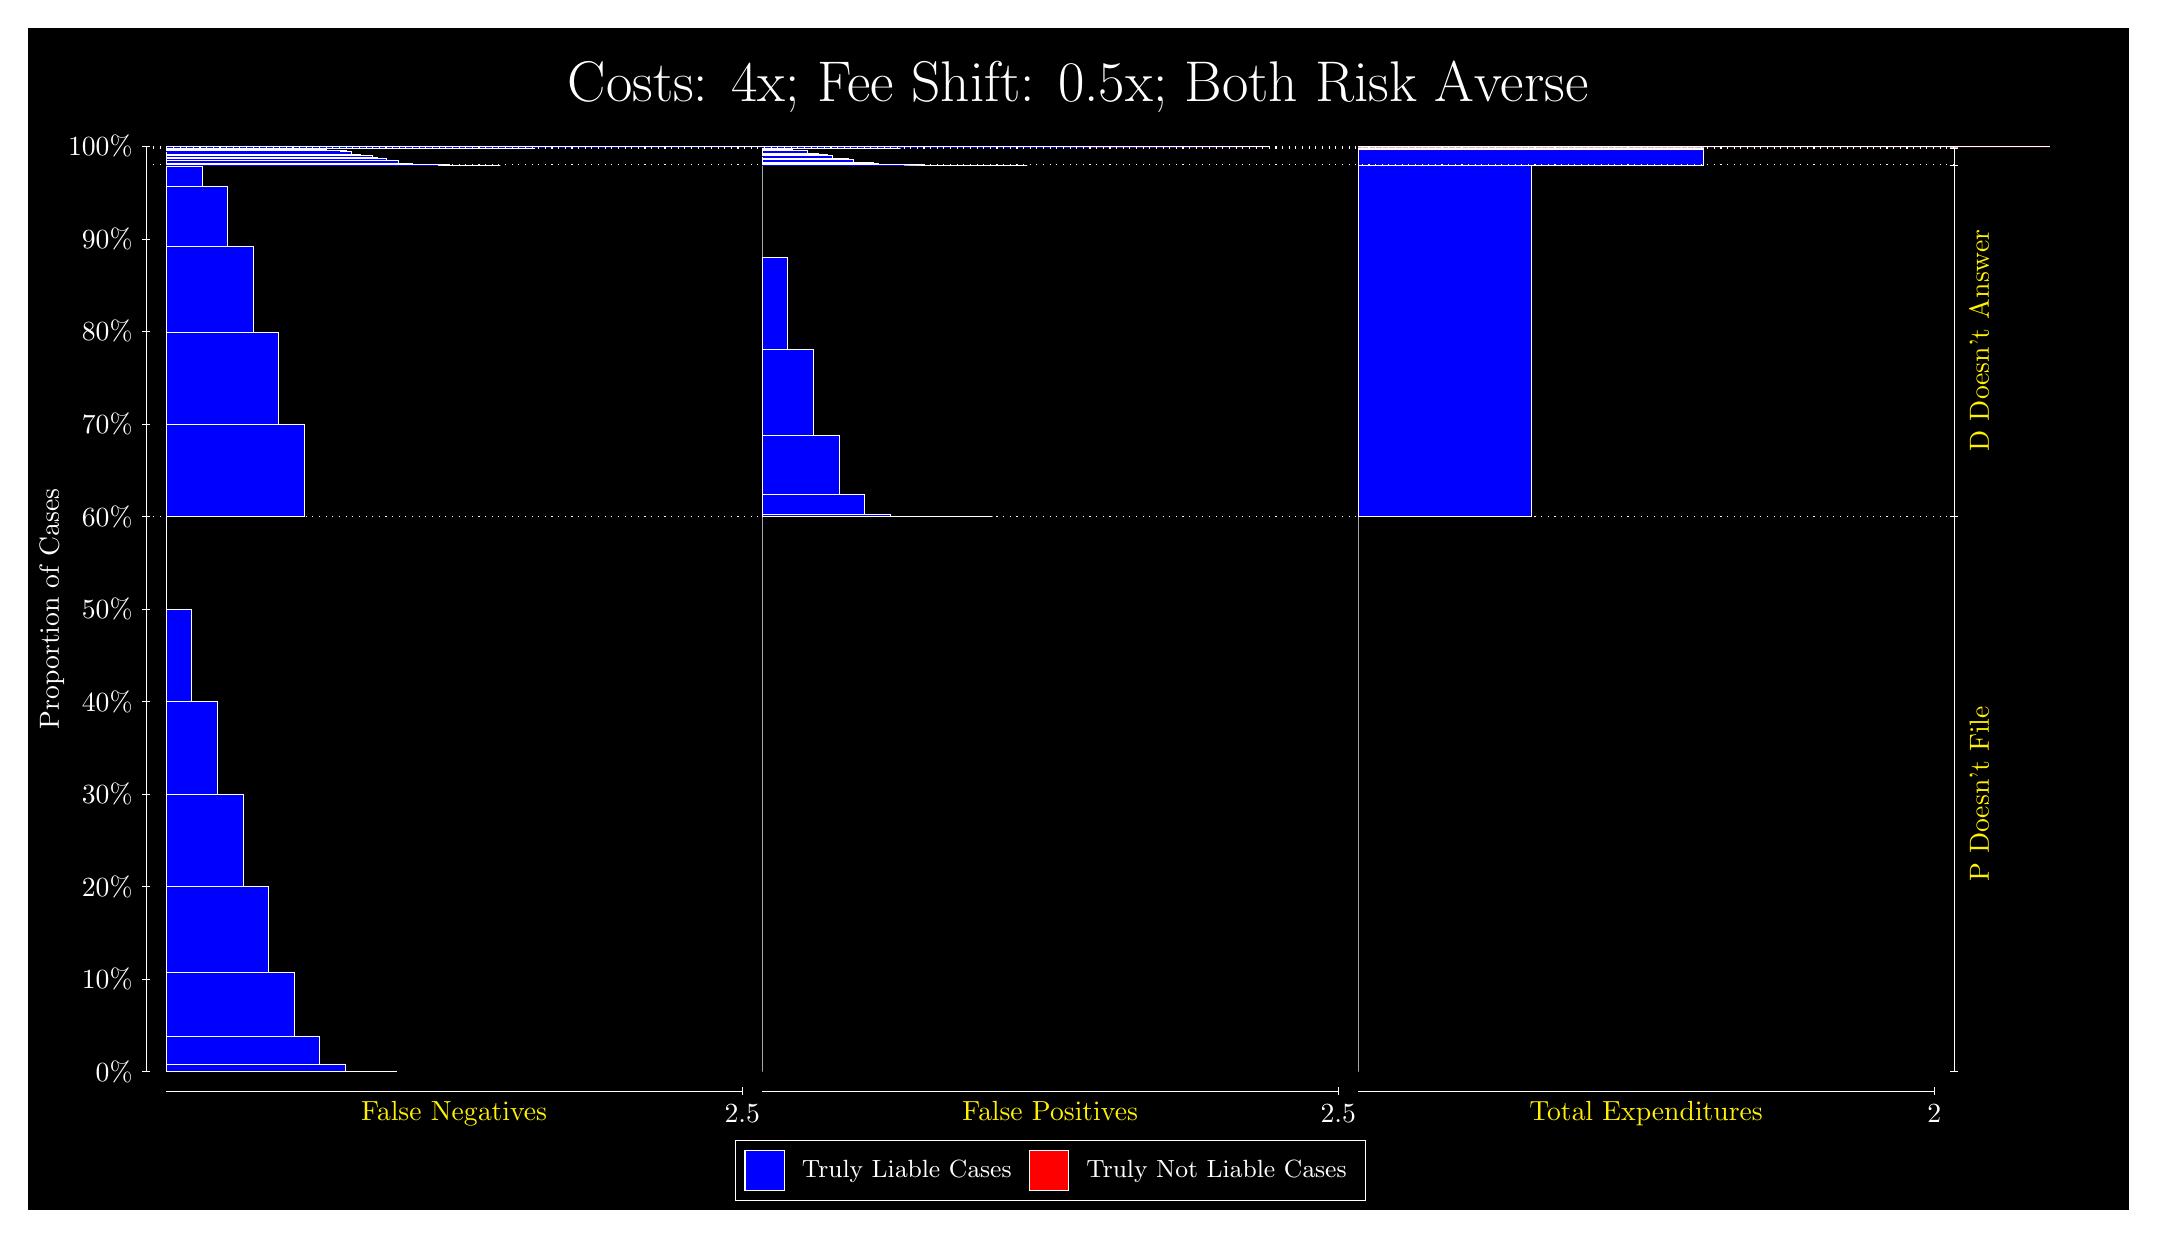
\begin{tikzpicture}
\draw[fill=black] (0,0) rectangle (26.667,15);
\draw[text=white] (0,13.5) rectangle (26.667,15) node[midway] {\huge Costs: 4x; Fee Shift: 0.5x; Both Risk Averse};
\draw[white, very thin] (1.5,1.75) -- (1.5,13.5);
\node[rotate=90, text=white, anchor=center] at (0.3, 7.625) {Proportion of Cases};
\draw[white, very thin] (1.45,1.75) -- (1.55,1.75);
\node[text=white, anchor=east] at (1.45, 1.75) {0\%};
\draw[white, very thin] (1.45,2.925) -- (1.55,2.925);
\node[text=white, anchor=east] at (1.45, 2.925) {10\%};
\draw[white, very thin] (1.45,4.1) -- (1.55,4.1);
\node[text=white, anchor=east] at (1.45, 4.1) {20\%};
\draw[white, very thin] (1.45,5.275) -- (1.55,5.275);
\node[text=white, anchor=east] at (1.45, 5.275) {30\%};
\draw[white, very thin] (1.45,6.45) -- (1.55,6.45);
\node[text=white, anchor=east] at (1.45, 6.45) {40\%};
\draw[white, very thin] (1.45,7.625) -- (1.55,7.625);
\node[text=white, anchor=east] at (1.45, 7.625) {50\%};
\draw[white, very thin] (1.45,8.8) -- (1.55,8.8);
\node[text=white, anchor=east] at (1.45, 8.8) {60\%};
\draw[white, very thin] (1.45,9.975) -- (1.55,9.975);
\node[text=white, anchor=east] at (1.45, 9.975) {70\%};
\draw[white, very thin] (1.45,11.15) -- (1.55,11.15);
\node[text=white, anchor=east] at (1.45, 11.15) {80\%};
\draw[white, very thin] (1.45,12.325) -- (1.55,12.325);
\node[text=white, anchor=east] at (1.45, 12.325) {90\%};
\draw[white, very thin] (1.45,13.5) -- (1.55,13.5);
\node[text=white, anchor=east] at (1.45, 13.5) {100\%};

\draw[white, very thin] (24.457,1.75) -- (24.457,13.5);
\draw[white, very thin] (24.407,1.75) -- (24.507,1.75);
\node[anchor=west] at (24.407, 1.75) {};
\draw[white, very thin] (24.407,8.8012) -- (24.507,8.8012);
\node[anchor=west] at (24.407, 8.8012) {};
\draw[white, very thin] (24.407,13.265) -- (24.507,13.265);
\node[anchor=west] at (24.407, 13.265) {};
\draw[white, very thin] (24.407,13.476) -- (24.507,13.476);
\node[anchor=west] at (24.407, 13.476) {};
\draw[white, very thin] (24.407,13.489) -- (24.507,13.489);
\node[anchor=west] at (24.407, 13.489) {};
\draw[white, very thin] (24.407,13.495) -- (24.507,13.495);
\node[anchor=west] at (24.407, 13.495) {};
\draw[white, very thin] (24.407,13.5) -- (24.507,13.5);
\node[anchor=west] at (24.407, 13.5) {};

\draw[white, very thin, fill=blue] (1.75,1.75) rectangle (4.6775,1.7504);
\draw[white, very thin, fill=blue] (1.75,1.7504) rectangle (4.3523,1.7582);
\draw[white, very thin, fill=blue] (1.75,1.7582) rectangle (4.027,1.8372);
\draw[white, very thin, fill=blue] (1.75,1.8372) rectangle (3.7017,2.1998);
\draw[white, very thin, fill=blue] (1.75,2.1998) rectangle (3.3764,3.0123);
\draw[white, very thin, fill=blue] (1.75,3.0123) rectangle (3.0511,4.1088);
\draw[white, very thin, fill=blue] (1.75,4.1088) rectangle (2.7258,5.2765);
\draw[white, very thin, fill=blue] (1.75,5.2765) rectangle (2.4006,6.4512);
\draw[white, very thin, fill=blue] (1.75,6.4512) rectangle (2.0753,7.6262);
\draw[white, very thin, fill=red] (1.75,7.6262) rectangle (1.75,7.6262);
\draw[white, very thin, fill=blue] (1.75,7.6262) rectangle (1.75,8.8012);
\draw[white, very thin, fill=blue] (1.75,8.8012) rectangle (3.5065,9.9758);
\draw[white, very thin, fill=blue] (1.75,9.9758) rectangle (3.1812,11.143);
\draw[white, very thin, fill=blue] (1.75,11.143) rectangle (2.856,12.232);
\draw[white, very thin, fill=blue] (1.75,12.232) rectangle (2.5307,12.99);
\draw[white, very thin, fill=blue] (1.75,12.99) rectangle (2.2054,13.241);
\draw[white, very thin, fill=blue] (1.75,13.241) rectangle (1.8801,13.265);
\draw[white, very thin, fill=red] (1.75,13.265) rectangle (1.75,13.265);
\draw[white, very thin, fill=blue] (1.75,13.265) rectangle (1.75,13.265);
\draw[white, very thin, fill=blue] (1.75,13.265) rectangle (5.9949,13.265);
\draw[white, very thin, fill=blue] (1.75,13.265) rectangle (5.8486,13.265);
\draw[white, very thin, fill=blue] (1.75,13.265) rectangle (5.7022,13.265);
\draw[white, very thin, fill=blue] (1.75,13.265) rectangle (5.6697,13.265);
\draw[white, very thin, fill=blue] (1.75,13.265) rectangle (5.5233,13.265);
\draw[white, very thin, fill=blue] (1.75,13.265) rectangle (5.4094,13.265);
\draw[white, very thin, fill=blue] (1.75,13.265) rectangle (5.3769,13.265);
\draw[white, very thin, fill=blue] (1.75,13.265) rectangle (5.3444,13.266);
\draw[white, very thin, fill=blue] (1.75,13.266) rectangle (5.2631,13.266);
\draw[white, very thin, fill=blue] (1.75,13.266) rectangle (5.198,13.267);
\draw[white, very thin, fill=blue] (1.75,13.267) rectangle (5.0842,13.267);
\draw[white, very thin, fill=blue] (1.75,13.267) rectangle (5.0516,13.267);
\draw[white, very thin, fill=blue] (1.75,13.267) rectangle (5.0191,13.278);
\draw[white, very thin, fill=blue] (1.75,13.278) rectangle (4.9378,13.278);
\draw[white, very thin, fill=blue] (1.75,13.278) rectangle (4.8727,13.286);
\draw[white, very thin, fill=blue] (1.75,13.286) rectangle (4.8239,13.286);
\draw[white, very thin, fill=blue] (1.75,13.286) rectangle (4.7589,13.287);
\draw[white, very thin, fill=blue] (1.75,13.287) rectangle (4.7263,13.288);
\draw[white, very thin, fill=blue] (1.75,13.288) rectangle (4.6938,13.325);
\draw[white, very thin, fill=blue] (1.75,13.325) rectangle (4.6125,13.325);
\draw[white, very thin, fill=blue] (1.75,13.325) rectangle (4.5474,13.344);
\draw[white, very thin, fill=blue] (1.75,13.344) rectangle (4.4986,13.344);
\draw[white, very thin, fill=blue] (1.75,13.344) rectangle (4.4336,13.361);
\draw[white, very thin, fill=blue] (1.75,13.361) rectangle (4.4011,13.361);
\draw[white, very thin, fill=blue] (1.75,13.361) rectangle (4.3685,13.39);
\draw[white, very thin, fill=blue] (1.75,13.39) rectangle (4.2872,13.391);
\draw[white, very thin, fill=blue] (1.75,13.391) rectangle (4.2222,13.398);
\draw[white, very thin, fill=blue] (1.75,13.398) rectangle (4.1734,13.4);
\draw[white, very thin, fill=blue] (1.75,13.4) rectangle (4.1083,13.439);
\draw[white, very thin, fill=blue] (1.75,13.439) rectangle (4.0758,13.439);
\draw[white, very thin, fill=blue] (1.75,13.439) rectangle (4.0432,13.444);
\draw[white, very thin, fill=blue] (1.75,13.444) rectangle (3.9619,13.445);
\draw[white, very thin, fill=blue] (1.75,13.445) rectangle (3.8969,13.446);
\draw[white, very thin, fill=blue] (1.75,13.446) rectangle (3.8481,13.453);
\draw[white, very thin, fill=blue] (1.75,13.453) rectangle (3.783,13.468);
\draw[white, very thin, fill=blue] (1.75,13.468) rectangle (3.7505,13.468);
\draw[white, very thin, fill=blue] (1.75,13.468) rectangle (3.718,13.468);
\draw[white, very thin, fill=blue] (1.75,13.468) rectangle (3.6366,13.468);
\draw[white, very thin, fill=blue] (1.75,13.468) rectangle (3.5716,13.468);
\draw[white, very thin, fill=blue] (1.75,13.468) rectangle (3.5228,13.474);
\draw[white, very thin, fill=blue] (1.75,13.474) rectangle (3.4577,13.475);
\draw[white, very thin, fill=blue] (1.75,13.475) rectangle (3.4252,13.475);
\draw[white, very thin, fill=blue] (1.75,13.475) rectangle (3.3927,13.475);
\draw[white, very thin, fill=blue] (1.75,13.475) rectangle (3.3114,13.475);
\draw[white, very thin, fill=blue] (1.75,13.475) rectangle (3.2463,13.475);
\draw[white, very thin, fill=blue] (1.75,13.475) rectangle (3.1975,13.476);
\draw[white, very thin, fill=blue] (1.75,13.476) rectangle (3.1325,13.476);
\draw[white, very thin, fill=blue] (1.75,13.476) rectangle (3.0999,13.476);
\draw[white, very thin, fill=blue] (1.75,13.476) rectangle (3.0674,13.476);
\draw[white, very thin, fill=blue] (1.75,13.476) rectangle (2.9861,13.476);
\draw[white, very thin, fill=blue] (1.75,13.476) rectangle (2.921,13.476);
\draw[white, very thin, fill=blue] (1.75,13.476) rectangle (2.8722,13.476);
\draw[white, very thin, fill=blue] (1.75,13.476) rectangle (2.8072,13.476);
\draw[white, very thin, fill=blue] (1.75,13.476) rectangle (2.7746,13.476);
\draw[white, very thin, fill=blue] (1.75,13.476) rectangle (2.6608,13.476);
\draw[white, very thin, fill=blue] (1.75,13.476) rectangle (2.5469,13.476);
\draw[white, very thin, fill=blue] (1.75,13.476) rectangle (2.4819,13.476);
\draw[white, very thin, fill=blue] (1.75,13.476) rectangle (2.3355,13.476);
\draw[white, very thin, fill=blue] (1.75,13.476) rectangle (2.2217,13.476);
\draw[white, very thin, fill=blue] (1.75,13.476) rectangle (1.8964,13.476);
\draw[white, very thin, fill=red] (1.75,13.476) rectangle (1.75,13.476);
\draw[white, very thin, fill=blue] (1.75,13.476) rectangle (6.4341,13.476);
\draw[white, very thin, fill=blue] (1.75,13.476) rectangle (6.1088,13.476);
\draw[white, very thin, fill=blue] (1.75,13.476) rectangle (5.7835,13.477);
\draw[white, very thin, fill=blue] (1.75,13.477) rectangle (5.4582,13.481);
\draw[white, very thin, fill=blue] (1.75,13.481) rectangle (5.1329,13.487);
\draw[white, very thin, fill=blue] (1.75,13.487) rectangle (4.8077,13.489);
\draw[white, very thin, fill=blue] (1.75,13.489) rectangle (4.4824,13.489);
\draw[white, very thin, fill=blue] (1.75,13.489) rectangle (4.1571,13.489);
\draw[white, very thin, fill=blue] (1.75,13.489) rectangle (3.8318,13.489);
\draw[white, very thin, fill=blue] (1.75,13.489) rectangle (3.5065,13.489);
\draw[white, very thin, fill=red] (1.75,13.489) rectangle (1.75,13.489);
\draw[white, very thin, fill=blue] (1.75,13.489) rectangle (3.5065,13.489);
\draw[white, very thin, fill=blue] (1.75,13.489) rectangle (3.1812,13.489);
\draw[white, very thin, fill=blue] (1.75,13.489) rectangle (2.856,13.49);
\draw[white, very thin, fill=blue] (1.75,13.49) rectangle (2.5307,13.493);
\draw[white, very thin, fill=blue] (1.75,13.493) rectangle (2.2054,13.495);
\draw[white, very thin, fill=blue] (1.75,13.495) rectangle (1.8801,13.495);
\draw[white, very thin, fill=red] (1.75,13.495) rectangle (1.75,13.495);
\draw[white, very thin, fill=blue] (1.75,13.495) rectangle (1.75,13.495);
\draw[white, very thin, fill=blue] (1.75,13.495) rectangle (9.9471,13.495);
\draw[white, very thin, fill=blue] (1.75,13.495) rectangle (9.6218,13.495);
\draw[white, very thin, fill=blue] (1.75,13.495) rectangle (9.2966,13.495);
\draw[white, very thin, fill=blue] (1.75,13.495) rectangle (8.9713,13.495);
\draw[white, very thin, fill=blue] (1.75,13.495) rectangle (8.646,13.495);
\draw[white, very thin, fill=blue] (1.75,13.495) rectangle (8.3207,13.495);
\draw[white, very thin, fill=blue] (1.75,13.495) rectangle (8.3207,13.495);
\draw[white, very thin, fill=blue] (1.75,13.495) rectangle (7.9954,13.495);
\draw[white, very thin, fill=blue] (1.75,13.495) rectangle (7.9954,13.495);
\draw[white, very thin, fill=blue] (1.75,13.495) rectangle (7.6702,13.495);
\draw[white, very thin, fill=blue] (1.75,13.495) rectangle (7.54,13.495);
\draw[white, very thin, fill=blue] (1.75,13.495) rectangle (7.3449,13.495);
\draw[white, very thin, fill=blue] (1.75,13.495) rectangle (7.3449,13.495);
\draw[white, very thin, fill=blue] (1.75,13.495) rectangle (7.2148,13.495);
\draw[white, very thin, fill=blue] (1.75,13.495) rectangle (7.0196,13.495);
\draw[white, very thin, fill=blue] (1.75,13.495) rectangle (6.8895,13.495);
\draw[white, very thin, fill=blue] (1.75,13.495) rectangle (6.6943,13.495);
\draw[white, very thin, fill=blue] (1.75,13.495) rectangle (6.5642,13.495);
\draw[white, very thin, fill=blue] (1.75,13.495) rectangle (6.369,13.495);
\draw[white, very thin, fill=blue] (1.75,13.495) rectangle (6.2389,13.495);
\draw[white, very thin, fill=blue] (1.75,13.495) rectangle (5.9136,13.496);
\draw[white, very thin, fill=blue] (1.75,13.496) rectangle (5.9136,13.496);
\draw[white, very thin, fill=blue] (1.75,13.496) rectangle (5.5883,13.497);
\draw[white, very thin, fill=blue] (1.75,13.497) rectangle (5.5883,13.497);
\draw[white, very thin, fill=blue] (1.75,13.497) rectangle (5.2631,13.498);
\draw[white, very thin, fill=blue] (1.75,13.498) rectangle (4.9378,13.499);
\draw[white, very thin, fill=blue] (1.75,13.499) rectangle (4.9378,13.499);
\draw[white, very thin, fill=blue] (1.75,13.499) rectangle (4.6125,13.499);
\draw[white, very thin, fill=blue] (1.75,13.499) rectangle (4.6125,13.5);
\draw[white, very thin, fill=blue] (1.75,13.5) rectangle (4.6125,13.5);
\draw[white, very thin, fill=blue] (1.75,13.5) rectangle (4.2872,13.5);
\draw[white, very thin, fill=blue] (1.75,13.5) rectangle (4.2872,13.5);
\draw[white, very thin, fill=blue] (1.75,13.5) rectangle (3.9619,13.5);
\draw[white, very thin, fill=blue] (1.75,13.5) rectangle (3.6366,13.5);
\draw[white, very thin, fill=blue] (1.75,13.5) rectangle (3.3114,13.5);
\draw[white, very thin, fill=blue] (1.75,13.5) rectangle (3.3114,13.5);
\draw[white, very thin, fill=blue] (1.75,13.5) rectangle (2.9861,13.5);
\draw[white, very thin, fill=blue] (1.75,13.5) rectangle (2.9861,13.5);
\draw[white, very thin, fill=blue] (1.75,13.5) rectangle (2.6608,13.5);
\draw[white, very thin, fill=blue] (1.75,13.5) rectangle (2.6608,13.5);
\draw[white, very thin, fill=blue] (1.75,13.5) rectangle (2.3355,13.5);
\draw[white, very thin, fill=red] (1.75,13.5) rectangle (1.75,13.5);
\draw[white, very thin, fill=red] (9.3189,1.75) rectangle (9.3189,1.75);
\draw[white, very thin, fill=blue] (9.3189,1.75) rectangle (9.3189,8.8012);
\draw[white, very thin, fill=red] (9.3189,8.8012) rectangle (12.246,8.8012);
\draw[white, very thin, fill=blue] (9.3189,8.8012) rectangle (12.246,8.8012);
\draw[white, very thin, fill=blue] (9.3189,8.8012) rectangle (11.921,8.8012);
\draw[white, very thin, fill=blue] (9.3189,8.8012) rectangle (11.596,8.8012);
\draw[white, very thin, fill=blue] (9.3189,8.8012) rectangle (11.271,8.8017);
\draw[white, very thin, fill=blue] (9.3189,8.8017) rectangle (10.945,8.8259);
\draw[white, very thin, fill=blue] (9.3189,8.8259) rectangle (10.62,9.0766);
\draw[white, very thin, fill=blue] (9.3189,9.0766) rectangle (10.295,9.8347);
\draw[white, very thin, fill=blue] (9.3189,9.8347) rectangle (9.9694,10.924);
\draw[white, very thin, fill=blue] (9.3189,10.924) rectangle (9.6442,12.091);
\draw[white, very thin, fill=blue] (9.3189,12.091) rectangle (9.3189,13.265);
\draw[white, very thin, fill=red] (9.3189,13.265) rectangle (12.686,13.265);
\draw[white, very thin, fill=blue] (9.3189,13.265) rectangle (12.686,13.265);
\draw[white, very thin, fill=blue] (9.3189,13.265) rectangle (12.36,13.265);
\draw[white, very thin, fill=red] (9.3189,13.265) rectangle (12.246,13.265);
\draw[white, very thin, fill=blue] (9.3189,13.265) rectangle (12.246,13.265);
\draw[white, very thin, fill=red] (9.3189,13.265) rectangle (12.1,13.265);
\draw[white, very thin, fill=blue] (9.3189,13.265) rectangle (12.1,13.265);
\draw[white, very thin, fill=blue] (9.3189,13.265) rectangle (12.035,13.265);
\draw[white, very thin, fill=blue] (9.3189,13.265) rectangle (11.921,13.265);
\draw[white, very thin, fill=red] (9.3189,13.265) rectangle (11.807,13.265);
\draw[white, very thin, fill=blue] (9.3189,13.265) rectangle (11.807,13.265);
\draw[white, very thin, fill=blue] (9.3189,13.265) rectangle (11.775,13.265);
\draw[white, very thin, fill=blue] (9.3189,13.265) rectangle (11.71,13.265);
\draw[white, very thin, fill=red] (9.3189,13.265) rectangle (11.661,13.265);
\draw[white, very thin, fill=blue] (9.3189,13.265) rectangle (11.661,13.265);
\draw[white, very thin, fill=blue] (9.3189,13.265) rectangle (11.596,13.265);
\draw[white, very thin, fill=red] (9.3189,13.265) rectangle (11.515,13.265);
\draw[white, very thin, fill=blue] (9.3189,13.265) rectangle (11.515,13.265);
\draw[white, very thin, fill=blue] (9.3189,13.265) rectangle (11.482,13.265);
\draw[white, very thin, fill=blue] (9.3189,13.265) rectangle (11.449,13.265);
\draw[white, very thin, fill=blue] (9.3189,13.265) rectangle (11.384,13.266);
\draw[white, very thin, fill=blue] (9.3189,13.266) rectangle (11.336,13.266);
\draw[white, very thin, fill=blue] (9.3189,13.266) rectangle (11.271,13.266);
\draw[white, very thin, fill=blue] (9.3189,13.266) rectangle (11.189,13.266);
\draw[white, very thin, fill=blue] (9.3189,13.266) rectangle (11.157,13.266);
\draw[white, very thin, fill=blue] (9.3189,13.266) rectangle (11.124,13.267);
\draw[white, very thin, fill=blue] (9.3189,13.267) rectangle (11.059,13.273);
\draw[white, very thin, fill=blue] (9.3189,13.273) rectangle (11.01,13.273);
\draw[white, very thin, fill=blue] (9.3189,13.273) rectangle (10.945,13.273);
\draw[white, very thin, fill=blue] (9.3189,13.273) rectangle (10.864,13.274);
\draw[white, very thin, fill=blue] (9.3189,13.274) rectangle (10.831,13.274);
\draw[white, very thin, fill=blue] (9.3189,13.274) rectangle (10.799,13.288);
\draw[white, very thin, fill=blue] (9.3189,13.288) rectangle (10.734,13.296);
\draw[white, very thin, fill=blue] (9.3189,13.296) rectangle (10.685,13.296);
\draw[white, very thin, fill=blue] (9.3189,13.296) rectangle (10.62,13.297);
\draw[white, very thin, fill=blue] (9.3189,13.297) rectangle (10.539,13.303);
\draw[white, very thin, fill=blue] (9.3189,13.303) rectangle (10.506,13.303);
\draw[white, very thin, fill=blue] (9.3189,13.303) rectangle (10.474,13.341);
\draw[white, very thin, fill=blue] (9.3189,13.341) rectangle (10.409,13.343);
\draw[white, very thin, fill=blue] (9.3189,13.343) rectangle (10.36,13.35);
\draw[white, very thin, fill=blue] (9.3189,13.35) rectangle (10.295,13.351);
\draw[white, very thin, fill=blue] (9.3189,13.351) rectangle (10.213,13.38);
\draw[white, very thin, fill=blue] (9.3189,13.38) rectangle (10.181,13.381);
\draw[white, very thin, fill=blue] (9.3189,13.381) rectangle (10.148,13.397);
\draw[white, very thin, fill=blue] (9.3189,13.397) rectangle (10.083,13.398);
\draw[white, very thin, fill=blue] (9.3189,13.398) rectangle (10.034,13.416);
\draw[white, very thin, fill=blue] (9.3189,13.416) rectangle (9.9694,13.416);
\draw[white, very thin, fill=blue] (9.3189,13.416) rectangle (9.8881,13.454);
\draw[white, very thin, fill=blue] (9.3189,13.454) rectangle (9.8556,13.454);
\draw[white, very thin, fill=blue] (9.3189,13.454) rectangle (9.8231,13.456);
\draw[white, very thin, fill=blue] (9.3189,13.456) rectangle (9.758,13.456);
\draw[white, very thin, fill=blue] (9.3189,13.456) rectangle (9.7092,13.464);
\draw[white, very thin, fill=blue] (9.3189,13.464) rectangle (9.6442,13.464);
\draw[white, very thin, fill=blue] (9.3189,13.464) rectangle (9.5628,13.474);
\draw[white, very thin, fill=blue] (9.3189,13.474) rectangle (9.5303,13.475);
\draw[white, very thin, fill=blue] (9.3189,13.475) rectangle (9.4978,13.475);
\draw[white, very thin, fill=blue] (9.3189,13.475) rectangle (9.3839,13.475);
\draw[white, very thin, fill=blue] (9.3189,13.475) rectangle (9.3189,13.476);
\draw[white, very thin, fill=red] (9.3189,13.476) rectangle (11.075,13.476);
\draw[white, very thin, fill=blue] (9.3189,13.476) rectangle (11.075,13.476);
\draw[white, very thin, fill=blue] (9.3189,13.476) rectangle (10.75,13.476);
\draw[white, very thin, fill=blue] (9.3189,13.476) rectangle (10.425,13.476);
\draw[white, very thin, fill=blue] (9.3189,13.476) rectangle (10.1,13.476);
\draw[white, very thin, fill=blue] (9.3189,13.476) rectangle (9.7743,13.478);
\draw[white, very thin, fill=blue] (9.3189,13.478) rectangle (9.449,13.484);
\draw[white, very thin, fill=blue] (9.3189,13.484) rectangle (9.3189,13.489);
\draw[white, very thin, fill=red] (9.3189,13.489) rectangle (14.003,13.489);
\draw[white, very thin, fill=blue] (9.3189,13.489) rectangle (14.003,13.489);
\draw[white, very thin, fill=blue] (9.3189,13.489) rectangle (13.678,13.489);
\draw[white, very thin, fill=blue] (9.3189,13.489) rectangle (13.352,13.489);
\draw[white, very thin, fill=blue] (9.3189,13.489) rectangle (13.027,13.489);
\draw[white, very thin, fill=blue] (9.3189,13.489) rectangle (12.702,13.489);
\draw[white, very thin, fill=blue] (9.3189,13.489) rectangle (12.377,13.491);
\draw[white, very thin, fill=blue] (9.3189,13.491) rectangle (12.051,13.494);
\draw[white, very thin, fill=blue] (9.3189,13.494) rectangle (11.726,13.495);
\draw[white, very thin, fill=blue] (9.3189,13.495) rectangle (11.401,13.495);
\draw[white, very thin, fill=blue] (9.3189,13.495) rectangle (11.075,13.495);
\draw[white, very thin, fill=red] (9.3189,13.495) rectangle (15.759,13.495);
\draw[white, very thin, fill=blue] (9.3189,13.495) rectangle (15.759,13.495);
\draw[white, very thin, fill=blue] (9.3189,13.495) rectangle (15.434,13.495);
\draw[white, very thin, fill=red] (9.3189,13.495) rectangle (15.434,13.495);
\draw[white, very thin, fill=blue] (9.3189,13.495) rectangle (15.434,13.495);
\draw[white, very thin, fill=red] (9.3189,13.495) rectangle (15.109,13.495);
\draw[white, very thin, fill=blue] (9.3189,13.495) rectangle (15.109,13.495);
\draw[white, very thin, fill=blue] (9.3189,13.495) rectangle (15.109,13.495);
\draw[white, very thin, fill=blue] (9.3189,13.495) rectangle (14.784,13.495);
\draw[white, very thin, fill=red] (9.3189,13.495) rectangle (14.784,13.495);
\draw[white, very thin, fill=blue] (9.3189,13.495) rectangle (14.784,13.495);
\draw[white, very thin, fill=blue] (9.3189,13.495) rectangle (14.784,13.495);
\draw[white, very thin, fill=blue] (9.3189,13.495) rectangle (14.458,13.495);
\draw[white, very thin, fill=red] (9.3189,13.495) rectangle (14.458,13.495);
\draw[white, very thin, fill=blue] (9.3189,13.495) rectangle (14.458,13.495);
\draw[white, very thin, fill=blue] (9.3189,13.495) rectangle (14.458,13.495);
\draw[white, very thin, fill=blue] (9.3189,13.495) rectangle (14.133,13.495);
\draw[white, very thin, fill=red] (9.3189,13.495) rectangle (14.133,13.495);
\draw[white, very thin, fill=blue] (9.3189,13.495) rectangle (14.133,13.495);
\draw[white, very thin, fill=blue] (9.3189,13.495) rectangle (14.133,13.495);
\draw[white, very thin, fill=blue] (9.3189,13.495) rectangle (13.808,13.495);
\draw[white, very thin, fill=blue] (9.3189,13.495) rectangle (13.808,13.495);
\draw[white, very thin, fill=red] (9.3189,13.495) rectangle (13.808,13.495);
\draw[white, very thin, fill=blue] (9.3189,13.495) rectangle (13.808,13.495);
\draw[white, very thin, fill=blue] (9.3189,13.495) rectangle (13.808,13.495);
\draw[white, very thin, fill=blue] (9.3189,13.495) rectangle (13.482,13.495);
\draw[white, very thin, fill=blue] (9.3189,13.495) rectangle (13.482,13.496);
\draw[white, very thin, fill=red] (9.3189,13.496) rectangle (13.482,13.496);
\draw[white, very thin, fill=blue] (9.3189,13.496) rectangle (13.482,13.496);
\draw[white, very thin, fill=blue] (9.3189,13.496) rectangle (13.157,13.496);
\draw[white, very thin, fill=blue] (9.3189,13.496) rectangle (13.157,13.497);
\draw[white, very thin, fill=blue] (9.3189,13.497) rectangle (13.157,13.497);
\draw[white, very thin, fill=blue] (9.3189,13.497) rectangle (12.832,13.498);
\draw[white, very thin, fill=blue] (9.3189,13.498) rectangle (12.832,13.498);
\draw[white, very thin, fill=blue] (9.3189,13.498) rectangle (12.832,13.498);
\draw[white, very thin, fill=blue] (9.3189,13.498) rectangle (12.507,13.499);
\draw[white, very thin, fill=blue] (9.3189,13.499) rectangle (12.507,13.499);
\draw[white, very thin, fill=blue] (9.3189,13.499) rectangle (12.507,13.499);
\draw[white, very thin, fill=blue] (9.3189,13.499) rectangle (12.181,13.499);
\draw[white, very thin, fill=blue] (9.3189,13.499) rectangle (12.181,13.5);
\draw[white, very thin, fill=blue] (9.3189,13.5) rectangle (12.181,13.5);
\draw[white, very thin, fill=blue] (9.3189,13.5) rectangle (11.856,13.5);
\draw[white, very thin, fill=blue] (9.3189,13.5) rectangle (11.856,13.5);
\draw[white, very thin, fill=blue] (9.3189,13.5) rectangle (11.856,13.5);
\draw[white, very thin, fill=red] (9.3189,13.5) rectangle (11.726,13.5);
\draw[white, very thin, fill=blue] (9.3189,13.5) rectangle (11.726,13.5);
\draw[white, very thin, fill=blue] (9.3189,13.5) rectangle (11.531,13.5);
\draw[white, very thin, fill=blue] (9.3189,13.5) rectangle (11.531,13.5);
\draw[white, very thin, fill=red] (9.3189,13.5) rectangle (11.401,13.5);
\draw[white, very thin, fill=blue] (9.3189,13.5) rectangle (11.401,13.5);
\draw[white, very thin, fill=blue] (9.3189,13.5) rectangle (11.206,13.5);
\draw[white, very thin, fill=blue] (9.3189,13.5) rectangle (11.206,13.5);
\draw[white, very thin, fill=red] (9.3189,13.5) rectangle (11.075,13.5);
\draw[white, very thin, fill=blue] (9.3189,13.5) rectangle (11.075,13.5);
\draw[white, very thin, fill=blue] (9.3189,13.5) rectangle (11.075,13.5);
\draw[white, very thin, fill=blue] (9.3189,13.5) rectangle (10.88,13.5);
\draw[white, very thin, fill=blue] (9.3189,13.5) rectangle (10.75,13.5);
\draw[white, very thin, fill=blue] (9.3189,13.5) rectangle (10.75,13.5);
\draw[white, very thin, fill=blue] (9.3189,13.5) rectangle (10.555,13.5);
\draw[white, very thin, fill=blue] (9.3189,13.5) rectangle (10.425,13.5);
\draw[white, very thin, fill=blue] (9.3189,13.5) rectangle (10.425,13.5);
\draw[white, very thin, fill=blue] (9.3189,13.5) rectangle (10.1,13.5);
\draw[white, very thin, fill=blue] (9.3189,13.5) rectangle (10.1,13.5);
\draw[white, very thin, fill=blue] (9.3189,13.5) rectangle (9.7743,13.5);
\draw[white, very thin, fill=blue] (9.3189,13.5) rectangle (9.7743,13.5);
\draw[white, very thin, fill=blue] (9.3189,13.5) rectangle (9.449,13.5);
\draw[white, very thin, fill=blue] (9.3189,13.5) rectangle (9.3189,13.5);
\draw[white, very thin, fill=red] (16.888,1.75) rectangle (16.888,1.75);
\draw[white, very thin, fill=blue] (16.888,1.75) rectangle (16.888,8.8012);
\draw[white, very thin, fill=red] (16.888,8.8012) rectangle (19.083,8.8012);
\draw[white, very thin, fill=blue] (16.888,8.8012) rectangle (19.083,13.265);
\draw[white, very thin, fill=red] (16.888,13.265) rectangle (21.279,13.265);
\draw[white, very thin, fill=blue] (16.888,13.265) rectangle (21.279,13.459);
\draw[white, very thin, fill=red] (16.888,13.459) rectangle (21.279,13.459);
\draw[white, very thin, fill=blue] (16.888,13.459) rectangle (21.279,13.476);
\draw[white, very thin, fill=red] (16.888,13.476) rectangle (21.279,13.476);
\draw[white, very thin, fill=blue] (16.888,13.476) rectangle (21.279,13.489);
\draw[white, very thin, fill=red] (16.888,13.489) rectangle (21.279,13.489);
\draw[white, very thin, fill=blue] (16.888,13.489) rectangle (21.279,13.495);
\draw[white, very thin, fill=red] (16.888,13.495) rectangle (25.67,13.495);
\draw[white, very thin, fill=blue] (16.888,13.495) rectangle (25.67,13.495);
\draw[white, very thin, fill=red] (16.888,13.495) rectangle (25.67,13.495);
\draw[white, very thin, fill=blue] (16.888,13.495) rectangle (25.67,13.499);
\draw[white, very thin, fill=red] (16.888,13.499) rectangle (25.67,13.499);
\draw[white, very thin, fill=blue] (16.888,13.499) rectangle (25.67,13.5);
\draw[white, dotted] (1.5,8.8012) -- (24.457,8.8012);
\draw[white, dotted] (1.5,13.265) -- (24.457,13.265);
\draw[white, dotted] (1.5,13.476) -- (24.457,13.476);
\draw[white, dotted] (1.5,13.489) -- (24.457,13.489);
\draw[white, dotted] (1.5,13.495) -- (24.457,13.495);
\draw[white, very thin] (1.75,1.5) -- (9.0689,1.5);
\node[text=yellow, anchor=north] at (5.4094, 1.5) {False Negatives};
\draw[white, very thin] (9.0689,1.45) -- (9.0689,1.55);
\node[text=white, anchor=north] at (9.0689, 1.45) {2.5};

\draw[white, very thin] (9.3189,1.5) -- (16.638,1.5);
\node[text=yellow, anchor=north] at (12.978, 1.5) {False Positives};
\draw[white, very thin] (16.638,1.45) -- (16.638,1.55);
\node[text=white, anchor=north] at (16.638, 1.45) {2.5};

\draw[white, very thin] (16.888,1.5) -- (24.207,1.5);
\node[text=yellow, anchor=north] at (20.547, 1.5) {Total Expenditures};
\draw[white, very thin] (24.207,1.45) -- (24.207,1.55);
\node[text=white, anchor=north] at (24.207, 1.45) {2};

\node[text=yellow, centered, rotate=90] at (24.777, 5.2756) {P Doesn't File};
\node[text=yellow, centered, rotate=90] at (24.777, 11.033) {D Doesn't Answer};





\draw (12.978300999999998,1.5) node[draw=none] (baseCoordinate) {};
\begin{scope}[align=center]
        \matrix[scale=0.5, draw=white, below=0.5cm of baseCoordinate, nodes={draw}, column sep=0.1cm]{
            \node[rectangle, draw, minimum width=0.5cm, minimum height=0.5cm, fill=blue] {}; &
            \node[draw=none, font=\small, text=white] (B) {Truly Liable Cases}; &
            \node[rectangle, draw, minimum width=0.5cm, minimum height=0.5cm, fill=red] {}; &
            \node[draw=none, font=\small, text=white] (B) {Truly Not Liable Cases}; \\
            };
\end{scope}

\end{tikzpicture}
\end{document}